\section{Current Sensing}
To address the difficulties of creating an accurate current-measurement circuit for cost-effective applications, designers have a variety of choices at their disposal. The best flexibility is provided by using general-purpose operational amplifiers (op amps) or analog-to-digital converters (ADCs), they could be standalone or embedded in a microcontroller (MCU). While also leveraging a wide range of tailored components that are specifically made for current sensing but also address challenges in a specific way \cite{TI_Current_Sensing}.
Shunt resistors(Kelvin method) and/or hall sensors are the two methods more widely used methods in automotive BMS applications to measure the battery pack current(Charging/Discharging and Balancing current). The integrated solutions for measuring current is more preferable, to secure the space and power constraints in automotive applications. The following sections will give more insights into the current sense methods.

\subsection{Hall Effect Current Sensors }
"The Hall effect is the creation of a voltage difference (the Hall voltage) across an electrical conductor that is transverse to an applied magnetic field perpendicular to the current and an electric current in the conductor". Well, that is a bit of a more scientific and deep mathematical explanation of the Hall effect. If I take a little leverage to explain the Hall effect in the nomenclature The Current flow in the conductor causes to induce magnetic flux inside the magnetic core, these fluxes also turn out a small potential, which can be called hall voltage. The Hall voltage dropped across the coil (Magnetic) is directionally proportional to the current flowing in the conductor.
A galvanically isolated Hall effect current sensor capable of DC or AC measurement with high accuracy, excellent linearity, and temperature stability\cite{TI_Hall_Current_Sensing_TMCS1107}.
Let us explore hall sensors with some typical examples in the BMS such as the TMCS1107xx \cite{TI_Hall_Current_Sensing_TMCS1107} series from the TI are the most popular and competitive galvanic solutions for measuring the current.

\subsubsection{TMCS1107xx Sensors :}
The TMCS1107-Q1 is a galvanically isolated Hall effect current sensor with high accuracy, great linearity, and temperature stability for measuring DC or AC currents. A signal chain with low drift and temperature compensation offers a $3\%$ full-scale error over the device temperature range.\\
A magnetic field is created by the input current flowing through an internal 1.8-m conductor, which is monitored by an integrated Hall-effect sensor. This topology reduces design complexity and does away with external concentrators. Reduced conductor resistance decreases thermal and power loss. A 420-V lifetime working voltage and a 3-kV RMS minimal isolation between the current path and circuitry are provided by inherent galvanic insulation. Transient immunity and high common-mode rejection are made possible by integrated electrical shielding. \\
The output voltage is proportional to the input current. Fixed sensitivity minimizes ratiometry errors and enhances supply noise rejection, enabling the TMCS1107-Q1 to run from a single 3-V to 5.5-V power supply. When current enters the positive input pin, it is regarded as having a positive polarity. There are options for both unidirectional and bidirectional sensing.\\
\begin{figure}[h]
	\centering
	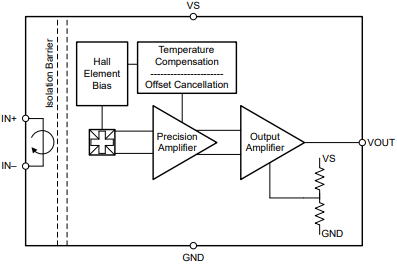
\includegraphics[width=0.8\textwidth]{Chap05/Figures/TMCS1107_HallSensor.PNG}
	\caption{TMCS1107xx Hall sensor Block diagram} 
	\label{fig:TMCS1107xx Hall sensor Block diagram}
\end{figure}
Input current to the TMCS1107-Q1 passes through the isolated side of the package lead frame through the
IN+ and IN– pins. The current flow through the package generates a magnetic field that is proportional to the
input current and measured by a galvanically isolated, precision, Hall sensor IC. As a result of the electrostatic
shielding on the Hall, sensor die, only the magnetic field generated by the input current is measured, thus limiting
input voltage switching pass-through to the circuitry\cite{TI_Hall_Current_Sensing_TMCS1107}.

